% generated by Plantuml 1.2022.7       
\definecolor{plantucolor0000}{RGB}{241,241,241}
\definecolor{plantucolor0001}{RGB}{24,24,24}
\definecolor{plantucolor0002}{RGB}{169,220,223}
\definecolor{plantucolor0003}{RGB}{0,0,0}
\definecolor{plantucolor0004}{RGB}{132,190,132}
\definecolor{plantucolor0005}{RGB}{3,128,72}
\definecolor{plantucolor0006}{RGB}{255,255,68}
\definecolor{plantucolor0007}{RGB}{179,141,34}
\definecolor{plantucolor0008}{RGB}{173,209,178}
\definecolor{plantucolor0009}{RGB}{200,41,48}
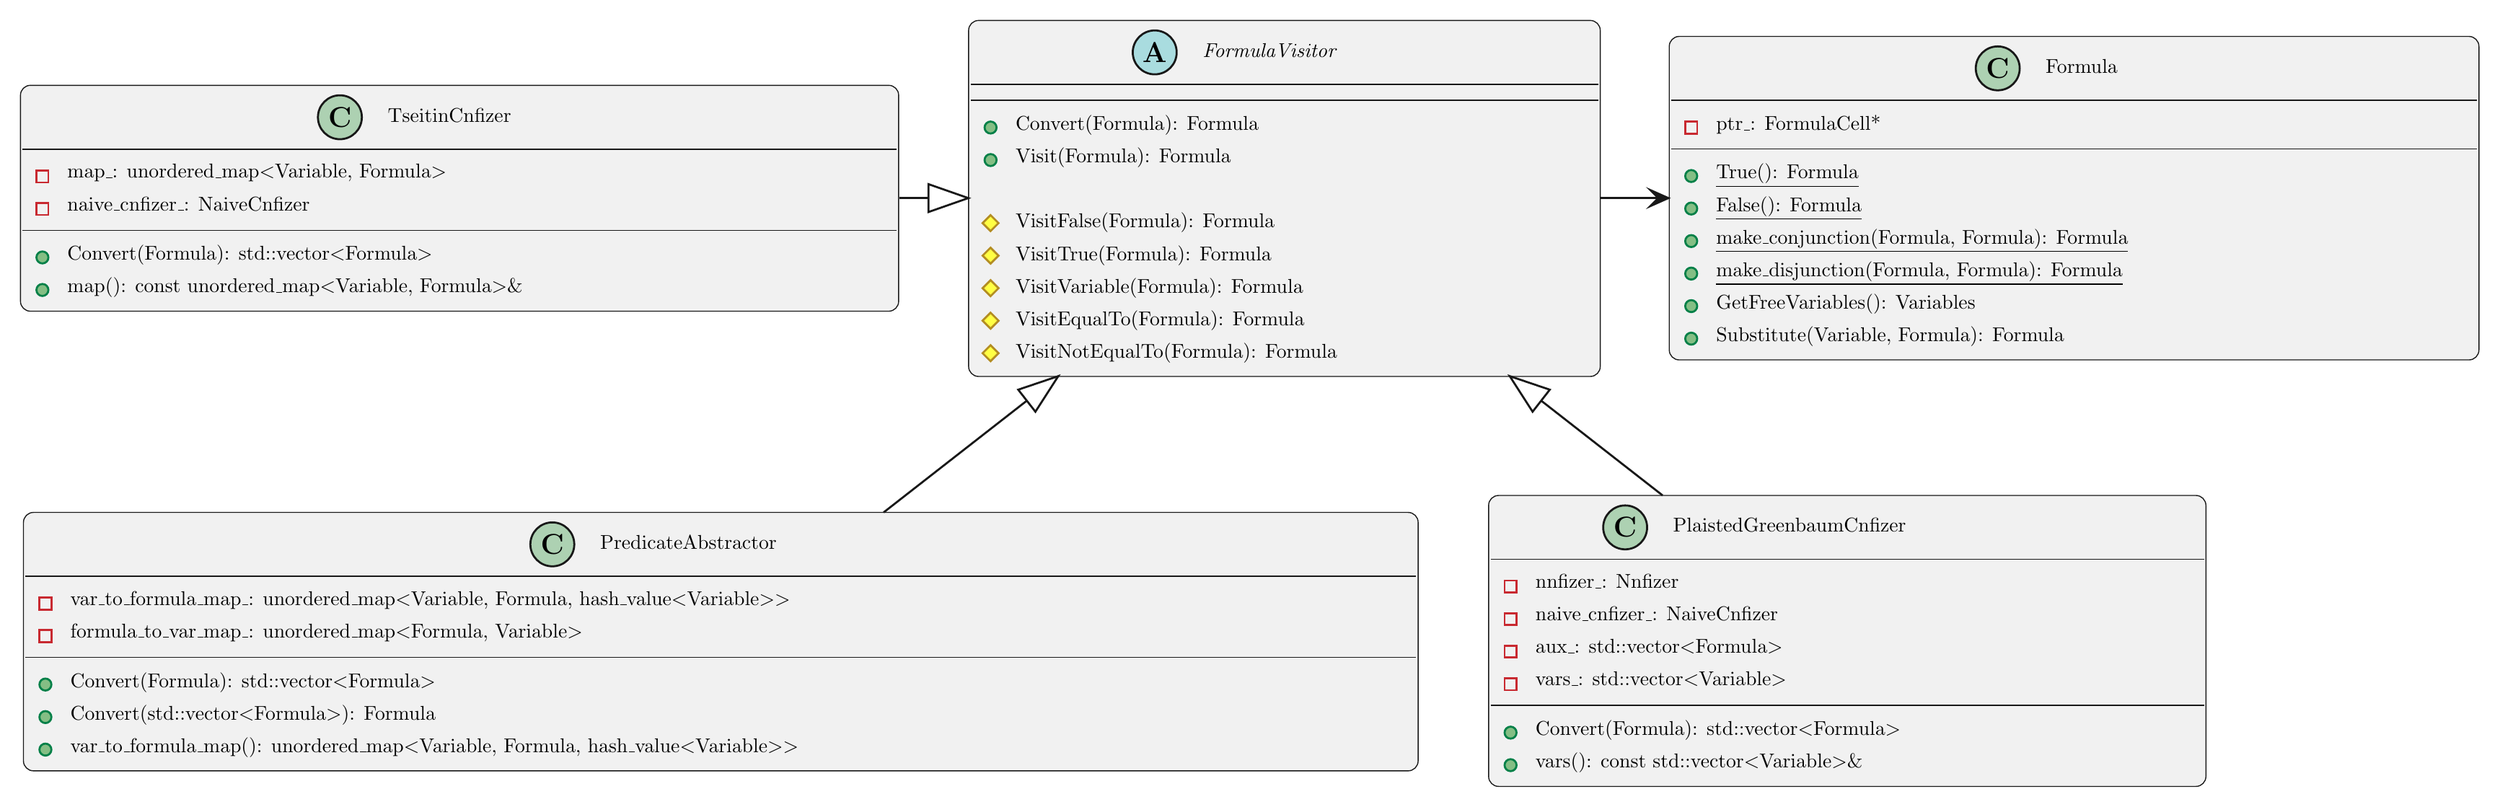
\begin{tikzpicture}[yscale=-1
,pstyle0/.style={color=plantucolor0001,fill=plantucolor0000,line width=0.5pt}
,pstyle2/.style={color=plantucolor0001,line width=0.5pt}
,pstyle3/.style={color=plantucolor0005,fill=plantucolor0004,line width=1.0pt}
,pstyle4/.style={color=plantucolor0007,fill=plantucolor0006,line width=1.0pt}
,pstyle5/.style={color=plantucolor0001,fill=plantucolor0008,line width=1.0pt}
,pstyle6/.style={color=plantucolor0009,line width=1.0pt}
,pstyle7/.style={color=plantucolor0001,line width=1.0pt}
]
\draw[pstyle0] (482pt,12pt) arc (180:270:5pt) -- (487pt,7pt) -- (793.43pt,7pt) arc (270:360:5pt) -- (798.43pt,12pt) -- (798.43pt,180.375pt) arc (0:90:5pt) -- (793.43pt,185.375pt) -- (487pt,185.375pt) arc (90:180:5pt) -- (482pt,180.375pt) -- cycle;
\draw[color=plantucolor0001,fill=plantucolor0002,line width=1.0pt] (575.2317pt,23pt) ellipse (11pt and 11pt);
\node at (575.2317pt,23pt)[]{\textbf{\Large A}};
\node at (595.7317pt,14.8516pt)[below right,color=black]{\textit{FormulaVisitor}};
\draw[pstyle2] (483pt,39pt) -- (797.43pt,39pt);
\draw[pstyle2] (483pt,47pt) -- (797.43pt,47pt);
\draw[pstyle3] (493pt,60.6484pt) ellipse (3pt and 3pt);
\node at (502pt,51pt)[below right,color=black]{Convert(Formula): Formula};
\draw[pstyle3] (493pt,76.9453pt) ellipse (3pt and 3pt);
\node at (502pt,67.2969pt)[below right,color=black]{Visit(Formula): Formula};
\node at (502pt,83.5938pt)[below right,color=black]{ };
\draw[pstyle4] (493pt,104.5391pt) -- (497pt,108.5391pt) -- (493pt,112.5391pt) -- (489pt,108.5391pt) -- cycle;
\node at (502pt,99.8906pt)[below right,color=black]{VisitFalse(Formula): Formula};
\draw[pstyle4] (493pt,120.8359pt) -- (497pt,124.8359pt) -- (493pt,128.8359pt) -- (489pt,124.8359pt) -- cycle;
\node at (502pt,116.1875pt)[below right,color=black]{VisitTrue(Formula): Formula};
\draw[pstyle4] (493pt,137.1328pt) -- (497pt,141.1328pt) -- (493pt,145.1328pt) -- (489pt,141.1328pt) -- cycle;
\node at (502pt,132.4844pt)[below right,color=black]{VisitVariable(Formula): Formula};
\draw[pstyle4] (493pt,153.4297pt) -- (497pt,157.4297pt) -- (493pt,161.4297pt) -- (489pt,157.4297pt) -- cycle;
\node at (502pt,148.7813pt)[below right,color=black]{VisitEqualTo(Formula): Formula};
\draw[pstyle4] (493pt,169.7266pt) -- (497pt,173.7266pt) -- (493pt,177.7266pt) -- (489pt,173.7266pt) -- cycle;
\node at (502pt,165.0781pt)[below right,color=black]{VisitNotEqualTo(Formula): Formula};
\draw[pstyle0] (8.5pt,258.5pt) arc (180:270:5pt) -- (13.5pt,253.5pt) -- (702.1973pt,253.5pt) arc (270:360:5pt) -- (707.1973pt,258.5pt) -- (707.1973pt,377.9844pt) arc (0:90:5pt) -- (702.1973pt,382.9844pt) -- (13.5pt,382.9844pt) arc (90:180:5pt) -- (8.5pt,377.9844pt) -- cycle;
\draw[pstyle5] (273.4486pt,269.5pt) ellipse (11pt and 11pt);
\node at (273.4486pt,269.5pt)[]{\textbf{\Large C}};
\node at (293.9486pt,261.3516pt)[below right,color=black]{PredicateAbstractor};
\draw[pstyle2] (9.5pt,285.5pt) -- (706.1973pt,285.5pt);
\draw[pstyle6] (16.5pt,296.1484pt) rectangle (22.5pt,302.1484pt);
\node at (28.5pt,289.5pt)[below right,color=black]{var\_to\_formula\_map\_: unordered\_map\textless Variable, Formula, hash\_value\textless Variable\textgreater \textgreater };
\draw[pstyle6] (16.5pt,312.4453pt) rectangle (22.5pt,318.4453pt);
\node at (28.5pt,305.7969pt)[below right,color=black]{formula\_to\_var\_map\_: unordered\_map\textless Formula, Variable\textgreater };
\draw[pstyle2] (9.5pt,326.0938pt) -- (706.1973pt,326.0938pt);
\draw[pstyle3] (19.5pt,339.7422pt) ellipse (3pt and 3pt);
\node at (28.5pt,330.0938pt)[below right,color=black]{Convert(Formula): std::vector\textless Formula\textgreater };
\draw[pstyle3] (19.5pt,356.0391pt) ellipse (3pt and 3pt);
\node at (28.5pt,346.3906pt)[below right,color=black]{Convert(std::vector\textless Formula\textgreater ): Formula};
\draw[pstyle3] (19.5pt,372.3359pt) ellipse (3pt and 3pt);
\node at (28.5pt,362.6875pt)[below right,color=black]{var\_to\_formula\_map(): unordered\_map\textless Variable, Formula, hash\_value\textless Variable\textgreater \textgreater };
\draw[pstyle0] (7pt,44.5pt) arc (180:270:5pt) -- (12pt,39.5pt) -- (441.9541pt,39.5pt) arc (270:360:5pt) -- (446.9541pt,44.5pt) -- (446.9541pt,147.6875pt) arc (0:90:5pt) -- (441.9541pt,152.6875pt) -- (12pt,152.6875pt) arc (90:180:5pt) -- (7pt,147.6875pt) -- cycle;
\draw[pstyle5] (167.0291pt,55.5pt) ellipse (11pt and 11pt);
\node at (167.0291pt,55.5pt)[]{\textbf{\Large C}};
\node at (187.5291pt,47.3516pt)[below right,color=black]{TseitinCnfizer};
\draw[pstyle2] (8pt,71.5pt) -- (445.9541pt,71.5pt);
\draw[pstyle6] (15pt,82.1484pt) rectangle (21pt,88.1484pt);
\node at (27pt,75.5pt)[below right,color=black]{map\_: unordered\_map\textless Variable, Formula\textgreater };
\draw[pstyle6] (15pt,98.4453pt) rectangle (21pt,104.4453pt);
\node at (27pt,91.7969pt)[below right,color=black]{naive\_cnfizer\_: NaiveCnfizer};
\draw[pstyle2] (8pt,112.0938pt) -- (445.9541pt,112.0938pt);
\draw[pstyle3] (18pt,125.7422pt) ellipse (3pt and 3pt);
\node at (27pt,116.0938pt)[below right,color=black]{Convert(Formula): std::vector\textless Formula\textgreater };
\draw[pstyle3] (18pt,142.0391pt) ellipse (3pt and 3pt);
\node at (27pt,132.3906pt)[below right,color=black]{map(): const unordered\_map\textless Variable, Formula\textgreater \&};
\draw[pstyle0] (742.5pt,250pt) arc (180:270:5pt) -- (747.5pt,245pt) -- (1096.8562pt,245pt) arc (270:360:5pt) -- (1101.8562pt,250pt) -- (1101.8562pt,385.7813pt) arc (0:90:5pt) -- (1096.8562pt,390.7813pt) -- (747.5pt,390.7813pt) arc (90:180:5pt) -- (742.5pt,385.7813pt) -- cycle;
\draw[pstyle5] (810.9071pt,261pt) ellipse (11pt and 11pt);
\node at (810.9071pt,261pt)[]{\textbf{\Large C}};
\node at (831.4071pt,252.8516pt)[below right,color=black]{PlaistedGreenbaumCnfizer};
\draw[pstyle2] (743.5pt,277pt) -- (1100.8562pt,277pt);
\draw[pstyle6] (750.5pt,287.6484pt) rectangle (756.5pt,293.6484pt);
\node at (762.5pt,281pt)[below right,color=black]{nnfizer\_: Nnfizer};
\draw[pstyle6] (750.5pt,303.9453pt) rectangle (756.5pt,309.9453pt);
\node at (762.5pt,297.2969pt)[below right,color=black]{naive\_cnfizer\_: NaiveCnfizer};
\draw[pstyle6] (750.5pt,320.2422pt) rectangle (756.5pt,326.2422pt);
\node at (762.5pt,313.5938pt)[below right,color=black]{aux\_: std::vector\textless Formula\textgreater };
\draw[pstyle6] (750.5pt,336.5391pt) rectangle (756.5pt,342.5391pt);
\node at (762.5pt,329.8906pt)[below right,color=black]{vars\_: std::vector\textless Variable\textgreater };
\draw[pstyle2] (743.5pt,350.1875pt) -- (1100.8562pt,350.1875pt);
\draw[pstyle3] (753.5pt,363.8359pt) ellipse (3pt and 3pt);
\node at (762.5pt,354.1875pt)[below right,color=black]{Convert(Formula): std::vector\textless Formula\textgreater };
\draw[pstyle3] (753.5pt,380.1328pt) ellipse (3pt and 3pt);
\node at (762.5pt,370.4844pt)[below right,color=black]{vars(): const std::vector\textless Variable\textgreater \&};
\draw[pstyle0] (833pt,20pt) arc (180:270:5pt) -- (838pt,15pt) -- (1233.6263pt,15pt) arc (270:360:5pt) -- (1238.6263pt,20pt) -- (1238.6263pt,172.0781pt) arc (0:90:5pt) -- (1233.6263pt,177.0781pt) -- (838pt,177.0781pt) arc (90:180:5pt) -- (833pt,172.0781pt) -- cycle;
\draw[pstyle5] (997.5632pt,31pt) ellipse (11pt and 11pt);
\node at (997.5632pt,31pt)[]{\textbf{\Large C}};
\node at (1018.0632pt,22.8516pt)[below right,color=black]{Formula};
\draw[pstyle2] (834pt,47pt) -- (1237.6263pt,47pt);
\draw[pstyle6] (841pt,57.6484pt) rectangle (847pt,63.6484pt);
\node at (853pt,51pt)[below right,color=black]{ptr\_: FormulaCell*};
\draw[pstyle2] (834pt,71.2969pt) -- (1237.6263pt,71.2969pt);
\draw[pstyle3] (844pt,84.9453pt) ellipse (3pt and 3pt);
\node at (853pt,75.2969pt)[below right,color=black]{\underline{True(): Formula}};
\draw[pstyle3] (844pt,101.2422pt) ellipse (3pt and 3pt);
\node at (853pt,91.5938pt)[below right,color=black]{\underline{False(): Formula}};
\draw[pstyle3] (844pt,117.5391pt) ellipse (3pt and 3pt);
\node at (853pt,107.8906pt)[below right,color=black]{\underline{make\_conjunction(Formula, Formula): Formula}};
\draw[pstyle3] (844pt,133.8359pt) ellipse (3pt and 3pt);
\node at (853pt,124.1875pt)[below right,color=black]{\underline{make\_disjunction(Formula, Formula): Formula}};
\draw[pstyle3] (844pt,150.1328pt) ellipse (3pt and 3pt);
\node at (853pt,140.4844pt)[below right,color=black]{GetFreeVariables(): Variables};
\draw[pstyle3] (844pt,166.4297pt) ellipse (3pt and 3pt);
\node at (853pt,156.7813pt)[below right,color=black]{Substitute(Variable, Formula): Formula};
\draw[pstyle7] (447.21pt,96pt) ..controls (452.08pt,96pt) and (456.96pt,96pt) .. (461.83pt,96pt);
\draw[pstyle7] (461.85pt,89pt) -- (481.85pt,96pt) -- (461.85pt,103pt) -- (461.85pt,89pt) -- cycle;
\draw[pstyle7] (769.01pt,197.64pt) ..controls (789.47pt,213.61pt) and (810.28pt,229.84pt) .. (829.68pt,244.98pt);
\draw[pstyle7] (764.54pt,203.04pt) -- (753.08pt,185.21pt) -- (773.15pt,192pt) -- (764.54pt,203.04pt) -- cycle;
\draw[pstyle7] (511.02pt,197.63pt) ..controls (486.66pt,216.63pt) and (461.81pt,236.01pt) .. (439.43pt,253.48pt);
\draw[pstyle7] (506.85pt,192pt) -- (526.92pt,185.21pt) -- (515.46pt,203.04pt) -- (506.85pt,192pt) -- cycle;
\draw[pstyle7] (798.17pt,96pt) ..controls (807.93pt,96pt) and (817.68pt,96pt) .. (827.44pt,96pt);
\draw[color=plantucolor0001,fill=plantucolor0001,line width=1.0pt] (832.54pt,96pt) -- (823.54pt,92pt) -- (827.54pt,96pt) -- (823.54pt,100pt) -- (832.54pt,96pt) -- cycle;
\end{tikzpicture}
